\sloppy
\chapter{DIZAJN INFORMACIONOG SISTEMA}

\sloppy
\section*{Kontrola verzija}


Zakir Šehić - opis arhitekturalnog paterna (razlozi, prednosti, mane)

\noindent Adnan Dervišević - dijagram komponenti i paketa, ERD dijagram

\noindent Zerina Ahmetović - prijedlog tehnologija za implementaciju

\noindent Tarik Hastor - UML tehnologija za implementaciju

\section{Arhitektura informacionog sistema}

U svrhu izgradnje informacionog sistema „Pozorište mladih“ odabrana je slojevita arhitektura, tačnije troslojna arhitektura, zbog njenih ključnih prednosti u podršci složenim i promjenjivim zahtjevima kulturnih institucija. Ovaj pristup dijeli sistem  na tri logička nivoa – nivo prezentacije, poslovni nivo i nivo pristupa podacima – čime se postiže efikasna organizacija resursa, veća prilagodljivost i dugoročna održivost.

\subsection{Razdvajanje odgovornosti}

Svaki nivo sistema ima jasno definisanu funkciju:
\begin{itemize}[label=\textbullet]
    \item \textbf{Nivo prezentacije} 

    
    Upravljanje vizualnim elementima i korisničkim interakcijama, kao što su rezervacija ulaznica i pregled programa putem interneta ili mobilnih aplikacija.
    \item \textbf{Poslovni nivo} 

    
    Sadrži sve funkcionalnosti i pravila sistema – od upravljanja rasporedom predstava i rezervacijama, do obračuna prihoda.
    \item \textbf{Nivo pristupa podacima} 

    
    Brine o pohrani, preuzimanju i integritetu informacija.
\end{itemize}
Ova jasna podjela omogućava da promjene u jednom dijelu sistema, kao što je izmjena dizajna web stranice, ne utiču na ostatak funkcionalnosti.

\subsection{Održivost i prilagodljivost}

Modularna struktura sistema omogućava ažuriranje bez rizika od lančanih grešaka. Na primjer, uvođenje novog načina plaćanja (kao što je integracija kriptovaluta) zahtijeva izmjene samo na poslovnom nivou, dok ostali dijelovi, poput korisničkog interfejsa i baze podataka, ostaju netaknuti. Ovo je od izuzetne važnosti za instituciju koja teži stalnom praćenju tehnoloških trendova i unapređenju ponude usluga.

\subsection{Skalabilnost}

Dizajn sistema omogućava prilagođavanje rastućem broju korisnika i podataka. U slučaju naglog porasta posjetitelja – na primjer, tokom kulturnih festivala – nivo prezentacije može se proširiti dodavanjem novih instanci, dok se baza podataka optimizira za brže pretrage. Na taj način osigurava se da performanse sistema ostanu na visokom nivou čak i pri velikom opterećenju.

\subsection{Tehnološka fleksibilnost}

Svaki nivo sistema može koristiti različite tehnologije, što omogućava izbor najprikladnijih alata za određene zadatke. Slobodan izbor tehnologija razvoja omogućavaju brzu prilagodbu novim trendovima, kao što su sistemi umjetne inteligencije za preporuke predstava ili napredna analitika posjeta.

\subsection{Testiranje}

Neovisno testiranje svakog nivoa značajno doprinosi pouzdanosti sistema:
\begin{itemize}[label=\textbullet]
    \item \textbf{\textit{Unit} testovi:} Testiranje poslovne logike omogućava simulaciju rezervacija bez pristupa stvarnoj bazi podataka.
    \item \textbf{Testovi performansi:} Analiza nivoa prezentacije može ukazati na uska grla, omogućavajući pravovremenu optimizaciju.
\end{itemize}

\Needspace{5\baselineskip} 
\subsection{Potencijalni izazovi i rješenja}
\begin{itemize}[label=\textbullet]
    \item \textbf{Kompleksnost komunikacije:} Upotreba API-ja između nivoa može uzrokovati kašnjenja. Ovo se može riješiti keširanjem često korištenih podataka i optimizacijom upita.
    \item \textbf{Ovisnost o jasno definiranim interfejsima:} Promjene u API-ju mogu narušiti stabilnost sistema, stoga je nužna detaljna dokumentacija i analiza istog.
\end{itemize}

\subsection{Uticaj novih IT trendova}

Novi trendovi u IT sektoru, kao što su cloud computing i serverless arhitektura, dodatno unapređuju prednosti troslojne arhitekture:

\subsubsection{Cloud computing – osnova skalabilnosti i fleksibilnosti}

\begin{itemize}[label=\textbullet]
    \item \textbf{Elastično skaliranje:} Prezentacijski nivo može se automatski proširivati u \textit{cloud-u} tokom razdoblja visoke posjećenosti, čime se smanjuju troškovi i poboljšavaju performanse.
    \item \textbf{Globalna dostupnost:} Resursi \textit{host-ovani} u više regija omogućavaju nižu latenciju za korisnike iz različitih dijelova svijeta.
    \item \textbf{Smanjenje operativnih troškova:} Upravljanje infrastrukturom preuzima \textit{cloud} pružatelj usluga, čime se omogućava da se razvojni tim fokusira na unaprjeđenje funkcionalnosti sistema.
\end{itemize}

\subsubsection{\textit{Serverless} arhitektura – revolucija u poslovnoj logici}

\begin{itemize}[label=\textbullet]
    \item \textbf{Obrada događaja:} Funkcije se aktiviraju isključivo na određene događaje (npr. rezervacija ulaznice), što doprinosi smanjenju troškova i povećanju efikasnosti.
    \item \textbf{Automatsko skaliranje:} \textit{Serverless} funkcije se automatski prilagođavaju opterećenju – na primjer, tokom masovne prodaje ulaznica sistem obrađuje veliki broj zahtjeva bez ručne intervencije.
    \item \textbf{Mikroservisni pristup:} Poslovna logika se razlaže na manje, neovisne funkcije, čime se poboljšava održivost i olakšava testiranje sistema.
\end{itemize}

\subsubsection{Prednosti za \textquotedblleft Pozorište Mladih\textquotedblright{}}

\begin{itemize}[label=\textbullet]
    \item \textbf{Ekonomska isplativost:} Model plaćanja po upotrebi kod \textit{serverless} rješenja (\textit{pay-per-use}) značajno smanjuje troškove u periodima nižeg opterećenja.
    \item \textbf{Brzina razvoja:} \textit{Cloud} servisi za autentifikaciju, ubrzavaju implementaciju novih funkcionalnosti, dok serverless pristup omogućava brzo puštanje u rad dodatnih funkcija.
    \item \textbf{Podrška za umjetnu inteligenciju i mašinsko učenje:} Cloud platforme nude unaprijed pripremljene modele za preporuke te napredne analitičke alate za praćenje posjeta.
\end{itemize}

\subsection{Dijagram komponenti i paketa}

\begin{figure}[H]
    \centering
    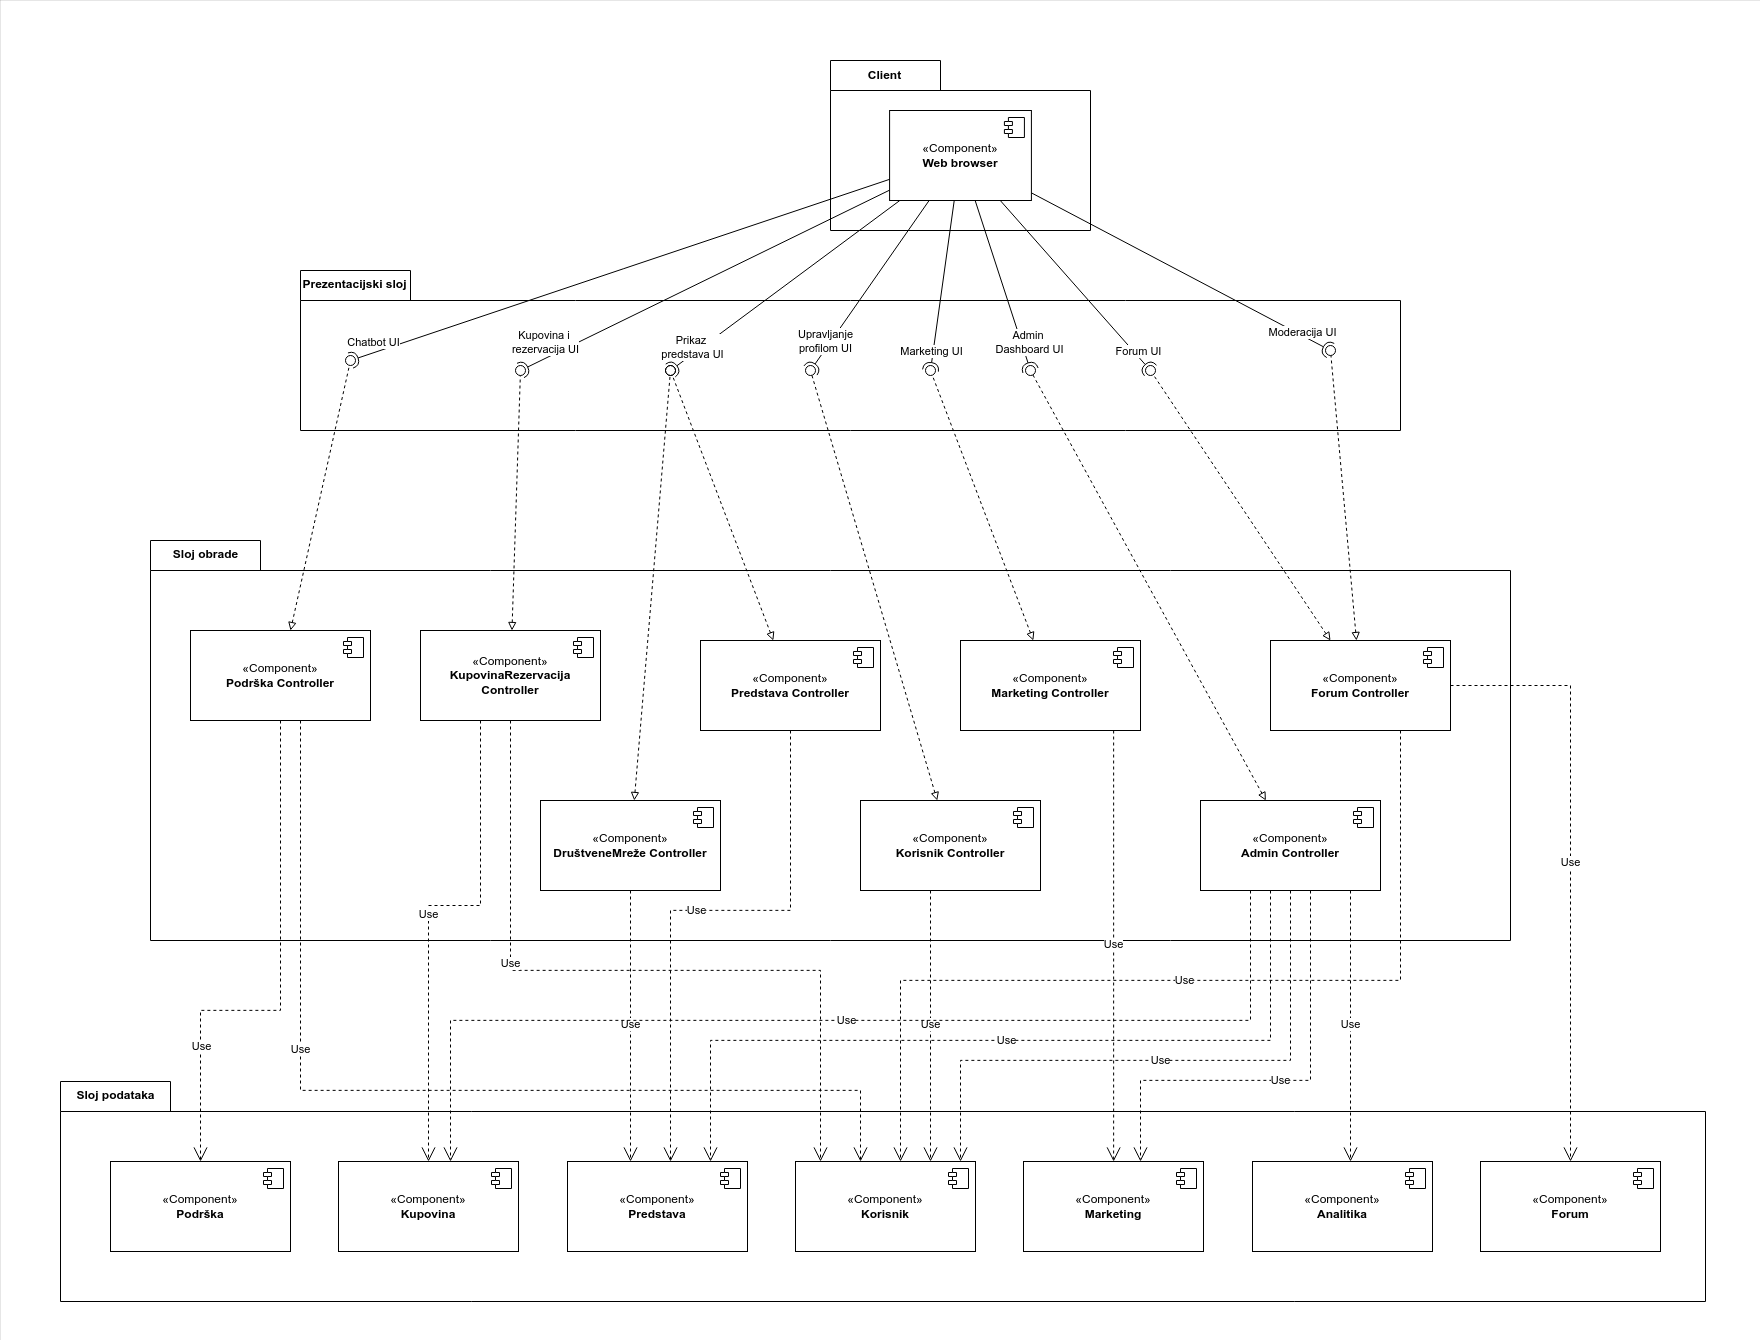
\includegraphics[width=0.9\textwidth]{Slike/Arhitektura/component.png}
    \caption{Dijagram komponenti i paketa}
    \label{fig:arh1}
\end{figure}

Na slici \ref{fig:arh1} je prikazan dijagram komponenti i paketa koji je dizajniran na osnovu funkcionalnih zahtjeva i jasno prikazuje troslojnu arhitekturu sistema.

\subsection{ERD dijagram}

\begin{figure}[H]
    \centering
    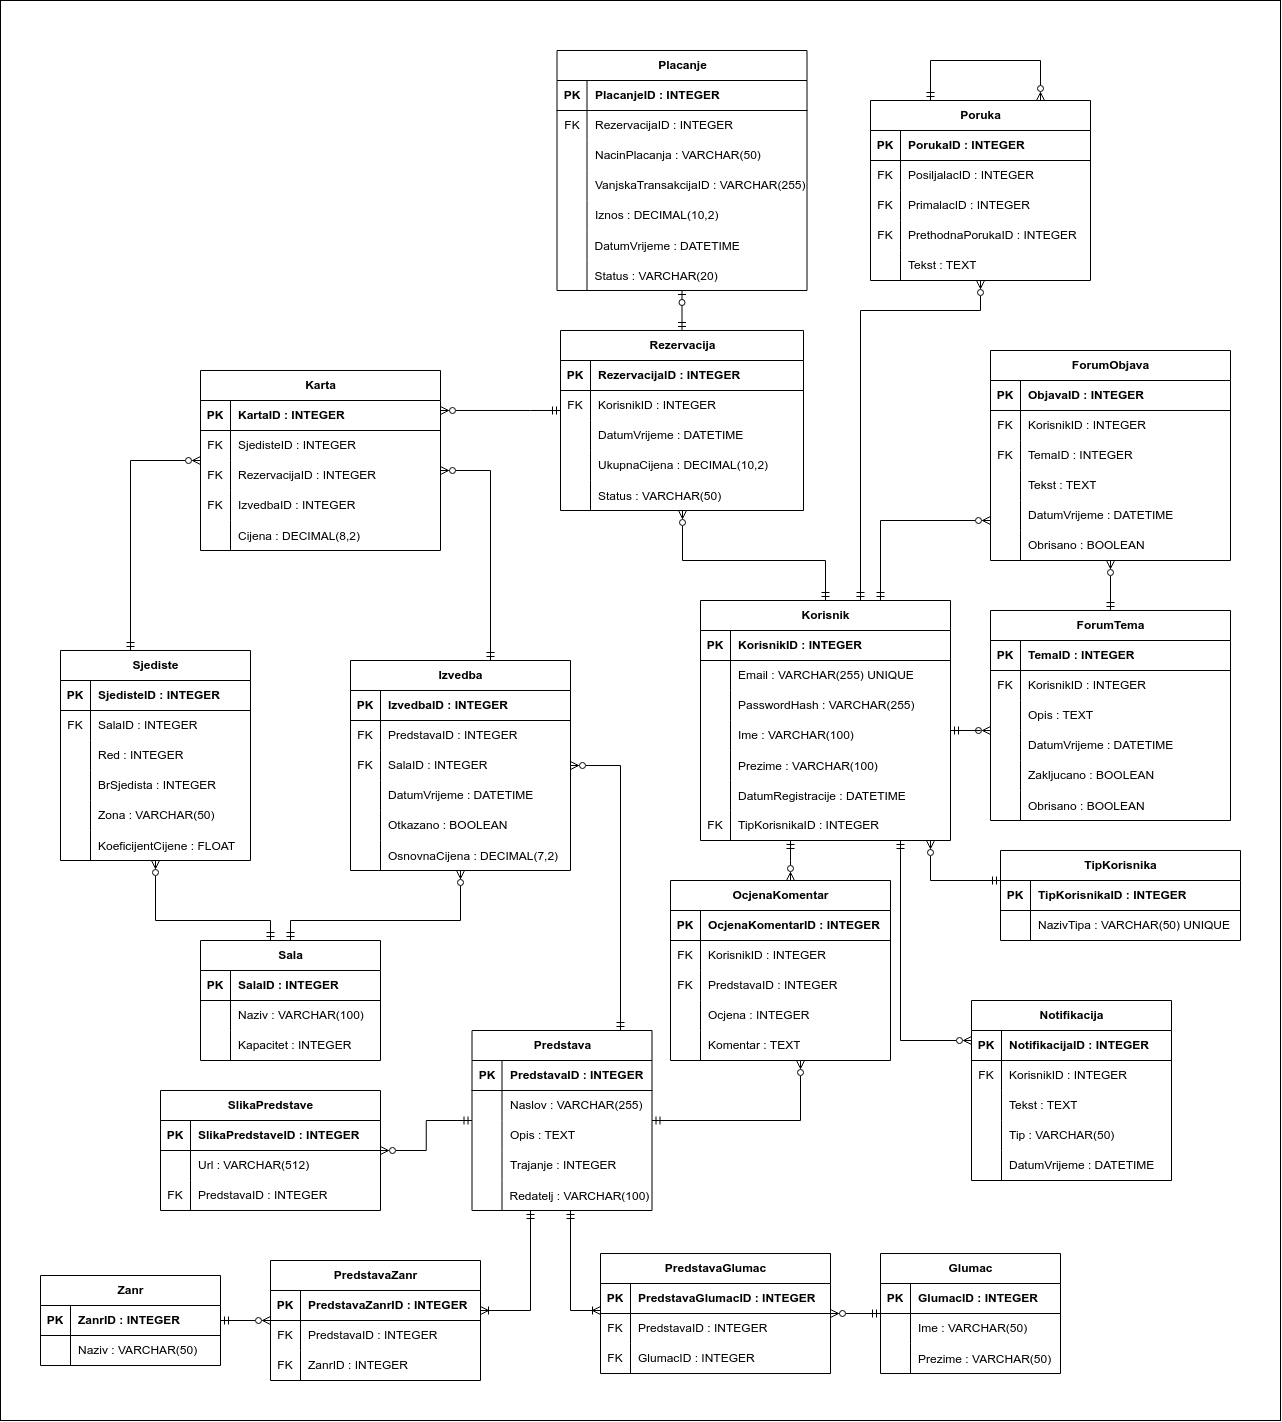
\includegraphics[width=0.8\textwidth]{Slike/Arhitektura/ERD.png}
    \caption{ERD dijagram}
    \label{fig:arh2}
\end{figure}

Na slici \ref{fig:arh2} je prikazan ERD dijagram koji modelira bazu podataka prema funkcionalnim zahtjevima.

\subsection{Zaključak}

Troslojna arhitektura predstavlja idealno rješenje za \textquotedblleft Pozorište Mladih\textquotedblright{} jer spaja performanse i skalabilnost, što je ključno za kulturne institucije usmjerene ka inovacijama i rastu. Ovaj model ne samo da zadovoljava trenutne zahtjeve, nego omogućava i laku tranziciju prema novim tehnologijama i poslovnim modelima, čime se sistem priprema za buduće izazove.

\section{Prijedlog tehnologija za implementaciju} \label{prijedlogTehnologijaZaImplementaciju}


\textbf{Prijedlog programskih jezika za komponente sistema:}
\begin{itemize}  
    \item \textbf{\textit{Frontend}}: \textit{JavaScript},te \textit{markup} jezici HTML, CSS

    
    Upotrebom \textit{JavaScript}-a se osigurava dinamičnost \textit{web} aplikacije, dok su HTML i CSS ključni pri strukturiranju i stilizaciji korisničkog interfejsa.
    \item \textbf{\textit{Backend} (serverska logika)}:  \textit{JavaScript}, uz\textit{ Node.js} okruženje

    
    \textit{Node.js} okruženje omogućava pisanje skalabilnih \textit{backend} servisa koristeći isti programski jezik kao na \textit{frontend} strani. Ovakav pristup uveliko olakšava razvoj sistema, kao i njegovo održavanje. 
    \item \textbf{Baza podataka}: \begin{itemize}
        \item \textbf{Jezik za upite:} SQL
        \item \textbf{Jezik za komunikaciju sa bazom:} \textit{JavaScript} (kroz \textit{Sequelize Object-Relational Mapping} - ORM)
    \end{itemize}
    Lahka integracija s \textit{Node.js backendom} i održava se dosljednost koda, budući da je isti programski jezik u upotrebi (\textit{JavaScript}). Ubrzava razvoj, koristan za brzu izradu protipa i lakšu migraciju baze.
\end{itemize} 
\textbf{Prijedlog \textit{framework}-a koji će se koristiti:}
\begin{itemize}  
    \item \textbf{Frontend}: \textit{React.js}

    
    \textit{React} nudi komponenti pristup razvoju korisničkog interfejsa, što olakšava održavanje i ponovno korištenje koda. Veće je brzine od njemu sličnih \textit{framework}-a, te ima širu zajednicu.
    \item \textbf{\textit{Backend} (serverska logika)}: \textit{Express.js} (unutar \textit{Node.js})

    
    \textit{Express} je minimalan i fleksibilan \textit{framework} koji omogućava brzo kreiranje REST API-ja i integraciju s različitim bazama podataka. Ima veliku zajednicu i mnoštvo dostupnih \textit{middleware} paketa.
\end{itemize} 
\textbf{Tip baze podataka:}
\begin{itemize}  
    \item \textbf{Relaciona baza podataka}: \textit{PostgreSQL}

    
    \textit{PostgreSQL} je \textit{open-source}, robustan i skalabilan sistem za upravljanje bazama podataka koji podržava kompleksne upite i transakcije. 
    
\end{itemize} 
\textbf{Eksterni web API servisi i protokoli:}
\begin{itemize}  
    \item \textbf{\textit{Payment Gateway} API}: \textit{Monri}, \textit{PayPal}\begin{itemize}
        \item \textbf{Namjena:} \textit{Online} plaćanje i fakturisanje.
        \item \textbf{Razlog:} Pouzdani, sigurni i široko korišteni servisi za obradu transakcija. \textit{Monri} je lokalno popularan, dok je \textit{PayPal} globalno.
    \end{itemize}
    \item \textbf{\textit{Google Maps} API} \begin{itemize}
        \item \textbf{Namjena:} Prikaz lokacije pozorišta.
        \item \textbf{Razlog:} Poboljšava korisničko iskustvo i olakšava dolazak posjetilaca.
    \end{itemize}
    \item \textbf{\textit{Social Media} API:} \textit{TikTok, Instagram} \begin{itemize}
        \item \textbf{Namjena:} Integracija sa društvenim mrežama u svrhu promocije predstava.
        \item \textbf{Razlog:} Omogućava automatsko objavljivanje sadržaja i promociju događaja.
    \end{itemize}
    \item \textbf{\textit{Firebase Cloud Messaging} (FCM)}\begin{itemize}
        \item \textbf{Namjena:} Slanje \textit{push} notifikacija korisnicima o predstojećim predstavama ili popustima.
        \item \textbf{Razlog:} Besplatan i lako integrisan servis za notifikacije.
    \end{itemize}
    \item \textbf{\textit{SendGrid }API ili \textit{Nodemailer} (za \textit{Email})} \begin{itemize}
        \item \textbf{Namjena:} Slanje potvrda o kupovini, promocija, izvještaja...
        \item \textbf{Razlog:} Pouzdana rješenja za slanje velikog broja \textit{email}-ova.
    \end{itemize}
    \item \textbf{\textit{Google Analytics}}\begin{itemize}
        \item \textbf{Namjena:} Prikupljanje podataka o ponašanju korisnika na platformi.
        \item \textbf{Razlog:} Važno za izvještavanje i optimizaciju poslovanja.
    \end{itemize}
\end{itemize} 
\textbf{Način pristupa sistemu (klijentska aplikacija):}
\begin{itemize}  
    \item \textbf{Web aplikacija}: \textit{index.}html učitan putem \textit{React} rutera (npr. /\textit{home}, /\textit{dashboard}, /\textit{login}) 
    Pristup kroz \textit{web browser} na desktopu i mobilnim uređajima.
\end{itemize} 
Navedeni prijedlog tehnologija prati osnovne principe troslojne arhitekture: \textbf{prezentacijski sloj (\textit{frontend})} realizovan je pomoću \textit{React} biblioteke i JavaScript jezika, poslovna logika (\textit{backend}) razvija se u \textit{Node.js }okruženju koristeći \textit{Express} \textit{framework}, dok se pristup podacima vrši preko \textit{Sequelize} ORM-a i \textit{PostgreSQL} baze podataka. Ovakav pristup omogućava jasno razdvajanje odgovornosti, bolju modularnost sistema, olakšano testiranje, kao i veću skalabilnost i održivost u budućnosti. Odabrane tehnologije međusobno su kompatibilne i odražavaju savremene industrijske standarde za razvoj \textit{web} aplikacija.

Na slici \ref{fig:arh3} je grafički prikaz ostvaren UML dijagramom raspoređivanja koji opisuje sve podsisteme i njihove najznačanije dijelove.

\begin{figure}[H]
    \centering
    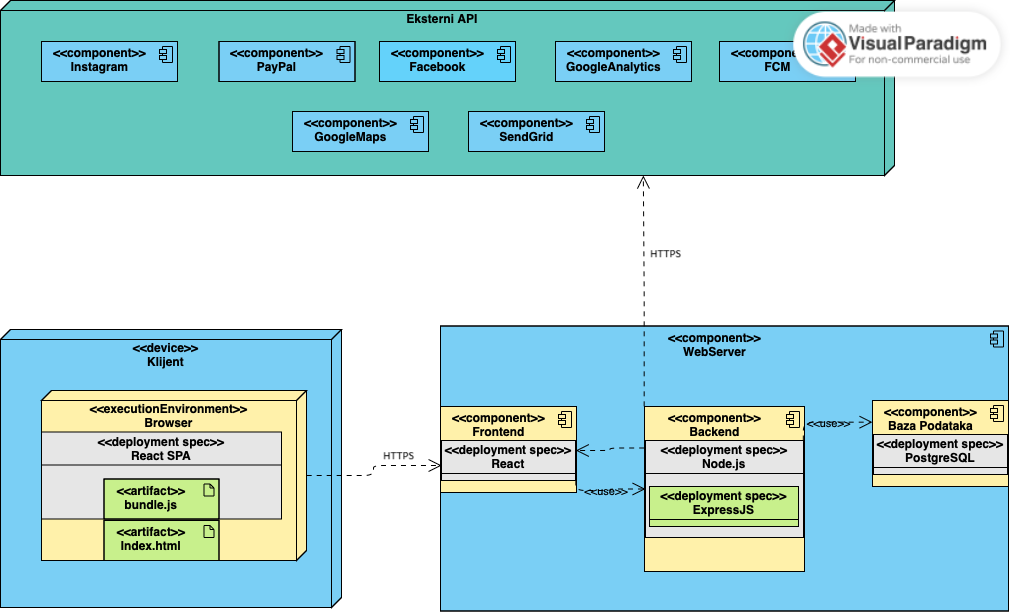
\includegraphics[width=0.8\textwidth]{Slike/Arhitektura/mrzimvpd.png}
    \caption{UML dijagram raspoređivanja}
    \label{fig:arh3}
\end{figure}

